\chapter{Goals and Use Cases}
\label{ch:Goals and Use Cases}

In this chapter, we discuss the intended goals of the project and list some use cases.

\section{Goals}

\paragraph{}
The goal of the project is to develop a software suite which facilitates interoperability between MANO frameworks, thereby enabling management of a network service across multi-vendor environments. To achieve this, we're dividing the software suite into 3 individual work packages (WP), which are developed in parallel initially and finally be merged. In the following sections, we discuss the individual goals of these modules in detail.

\subsection{Service Descriptor Translator (SDT)}
\paragraph{}

In this work package we implement a translator engine for a Network Service Descriptor (NSD). The Network Function Virtualization Orchestrator (NFVO) is the main orchestration unit of a MANO framework that manages the lifecycle of a network service (NS). One of the main functions of a NFVO is registering a network service in the NS catalog by onboarding the NSD. In a scenario where a network service needs to be deployed and registered among two different MANO
frameworks having their own NSD schema, our translator engine would help translate the NSD schema from one MANO framework to the other.
We will have mechanisms to extract the NSD schema from the NS catalog of the two different MANO frameworks and pass it to SDT engine which will consume the NSD schemas and translate one NSD schema to the other MANO framework's NSD schema. REST interfaces will be made available for other services to interface with the SDT.

\subsection{Service Descriptor Splitter (SDS)}
\paragraph{}

In production environment, a Network Service will be deployed over a vast geographical region and will span multiple domains, in such scenarios there is a need to split a Network Service into smaller network services and deploy it over multiple domains. In this work package we implement a Service Descriptor Splitter (SDS) which will be splitting the NSD of NS. SDS will be taking NSD as an input which will have all the information elements which can be extracted to generate separate NSDs. In our approach, the Service Graph is extracted from the input NSD and is split into subgraphs which will result in a separate set of elements such as Virtual Network Functions, Virtual Links, Virtual Network Function Forwarding Graphs etc. We will be evaluating different network graph splitting algorithms to split the Service graph. We will take these sets and generate NSDs according to the domain specific orchestrators.

\begin{figure}[h]
	\centering
	\includegraphics[width=0.7\linewidth]{figures/splitter_diagram}
	\caption{This figure visualizes the structure of SDS work package. }
	\label{fig:splitterDiagram}
\end{figure}

\subsection{MANO Adaptor (MA)}
\paragraph{}

A key component of a MANO framework is Virtualized Interface Manager (VIM),  which helps in assigning the hardware resources to virtual resources. The MANO framework uses specific adaptors to communicate with their respective VIMs. For instance, Sonata \ref{SecSONATA} MANO framework has adaptors for OpenStack \ref{label} and Kubernetes\ref{label}. However, when there is a spike in the service request beyond the capabilities of a single MANO instance, multiple MANO instances should be instantiated to balance the load. The goal of this work package is to build an adaptor that facilitates interaction between different instances of MANO frameworks, thereby exposing the underlying MANO framework's interfaces and enabling monitoring of the underlying service states.

\paragraph{}
Apart from the implementation of MA, we are planning to investigate MANO scalability challenges by answering research questions such as the ones listed below but not limited to.
\begin{itemize}
	\item What is the optimal number of MANO instances in a system?
	\item What is the optimal hierarchical level in a system?
\end{itemize}


\subsection{Integration Of Work Packages}
\paragraph{}

In this work package we integrate the translator engine, splitter engine and the MANO adaptor. This integration will augment the funtionality of the MANO adaptor in terms of addressing the scalability challenges between different MANO frameworks. It also extends the capability of both the splitter engine and translator engine to split a NSD and then deploy a part of it to a different MANO framework. All these individual modules are planned to be implemented as microservices and integrated keeping their individual autonomy intact. 

\begin{figure}[h]
	\centering
	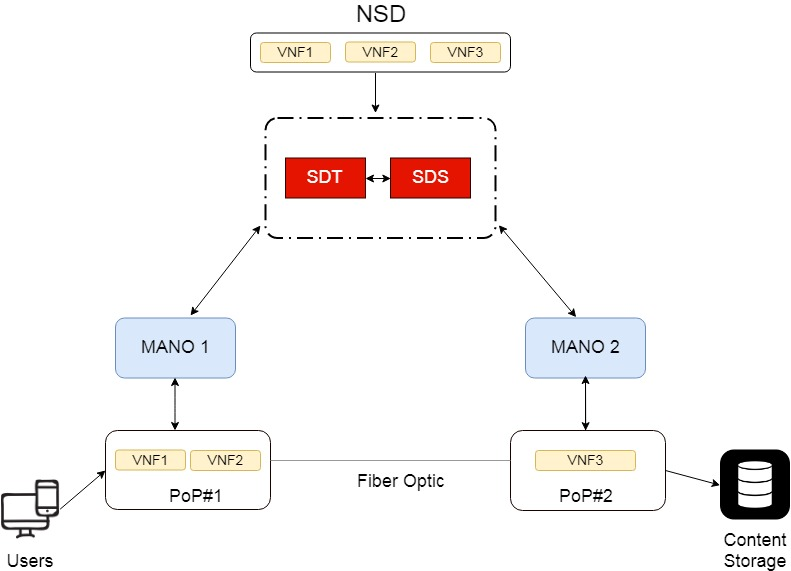
\includegraphics[width=0.7\linewidth]{figures/Structure1}
	\caption{This figure visualizes the structure of first and second modules. }
	\label{fig:structure1}
\end{figure}

\begin{figure}[h]
	\centering
	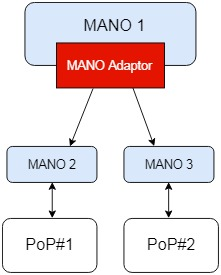
\includegraphics[width=0.3\linewidth]{figures/Structure2}
	\caption{This figure visualizes the structure of third module. }
	\label{fig:structure2}
\end{figure}

\paragraph{}
The project group will be initially divided into 3 subgroups. Each subgroup works on a single work package. However, update on work in progress and knowledge transfer will continuously take place between the subgroups. In the final development phase, the entire team will work towards integrating the individual modules of the work packages into a single software suite.

\newpage
\section{Use Cases}

\subsection{Cross-MANO Framework Interaction}
\paragraph{}

The MANO frameworks used by every network service provider varies from one another. NSD translation enables the deployment of network services that is in accordance with the intended framework.

For instance: Consider two Network Service Operators using different MANO frameworks. One of them uses Sonata framework \cite{draxler2017sonata} and another operator uses OSM framework \cite{ersue2013etsi}. These frameworks have different NSD schemata(refer \ref{SecSONATA} and \ref{SecOSM}). NSD schemata contains VNFs, virtual links, and VNF forwarding graphs and also describes the deployment of a Network Service. By using a translator, these NSD schemata can be translated to framework-specific schema. With this, operators can deploy and manage Network Services across different MANO implementations.

\subsection{Hierarchical Orchestration}
\paragraph{}
By using the MANO adapter, dynamic instantiation of multiple MANO instances and inter-operability between different MANO frameworks can be achieved. The operator will be able to handle the resources in an efficient manner, as one MANO framework can manage a limited number of service requests, operators can explore options to include additional MANO instances under the existing MANO instance to mitigate the traffic load on a single instance. The resources can be provisioned based on the number of requests. This helps the operator in extending their profitability.
\newpage
\textbf{Actors} : The Network Service Providers who would use features of SCrAMbLE.

\begin{figure} [h]
	\centering
	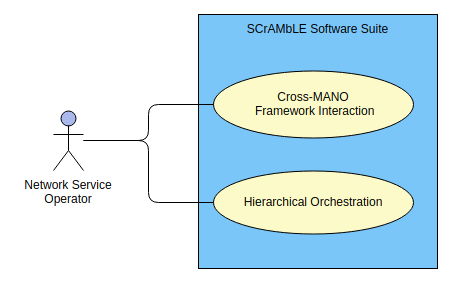
\includegraphics[width=1.0\linewidth]{figures/use-case}
	\caption{Use Case Diagram}
	\label{fig:use-case}
\end{figure}





